% !TeX program = pdfLaTeX
\documentclass[12pt]{article}
\usepackage{amsmath}
\usepackage{graphicx,psfrag,epsf}
\usepackage{enumerate}
\usepackage{natbib}
\usepackage{textcomp}
\usepackage[hyphens]{url} % not crucial - just used below for the URL
\usepackage{hyperref}

%\pdfminorversion=4
% NOTE: To produce blinded version, replace "0" with "1" below.
\newcommand{\blind}{0}

% DON'T change margins - should be 1 inch all around.
\addtolength{\oddsidemargin}{-.5in}%
\addtolength{\evensidemargin}{-.5in}%
\addtolength{\textwidth}{1in}%
\addtolength{\textheight}{1.3in}%
\addtolength{\topmargin}{-.8in}%

%% load any required packages here



% tightlist command for lists without linebreak
\providecommand{\tightlist}{%
  \setlength{\itemsep}{0pt}\setlength{\parskip}{0pt}}



\usepackage{amsmath}
\usepackage{amsfonts}
\usepackage{booktabs}
\usepackage{makecell}
\usepackage[usenames, dvipsnames]{color}
\usepackage{multirow}
\usepackage{comment}
\usepackage{booktabs}
\usepackage{longtable}
\usepackage{array}
\usepackage{wrapfig}
\usepackage{float}
\usepackage{colortbl}
\usepackage{pdflscape}
\usepackage{tabu}
\usepackage{threeparttable}
\usepackage{threeparttablex}
\usepackage[normalem]{ulem}
\usepackage{xcolor}
\newcommand{\beginsupplement}{\setcounter{table}{0} \renewcommand{\thetable}{S\arabic{table}}\setcounter{figure}{0} \renewcommand{\thefigure}{S\arabic{figure}}}

\begin{document}


\def\spacingset#1{\renewcommand{\baselinestretch}%
{#1}\small\normalsize} \spacingset{1}


%%%%%%%%%%%%%%%%%%%%%%%%%%%%%%%%%%%%%%%%%%%%%%%%%%%%%%%%%%%%%%%%%%%%%%%%%%%%%%

\if0\blind
{
  \title{\bf Climate Migration Amplifies Demographic Change and
Population Aging}

  \author{
        Mathew E. Hauer \thanks{Thanks y'all!} \\
    Department of Sociology, Florida State University\\
     and \\     Sunshine Jacobs \\
    Department of Sociology, Florida State University\\
     and \\     Scott Kulp \\
    Climate Central\\
      }
  \maketitle
} \fi

\if1\blind
{
  \bigskip
  \bigskip
  \bigskip
  \begin{center}
    {\LARGE\bf Climate Migration Amplifies Demographic Change and
Population Aging}
  \end{center}
  \medskip
} \fi

\bigskip
\begin{abstract}
The warnings of potential climate migration first appeared in the
scientific literature in the late 1970s when increased recognition that
disintegrating ice sheets could drive people to migrate from coastal
cities. Since that time, scientists have modelled potential climate
migration without integrating other population processes, potentially
obscuring the demographic amplification of this migration. Climate
migration could amplify demographic change -- enhancing migration to
destinations and suppressing migration to origins. Additionally, older
populations are the least likely to migrate and climate migration could
accelerate population aging in origin areas. Here, we investigate
climate migration under sea-level rise (SLR), a single climatic hazard,
and examine both the potential demographic amplification effect and
population aging by combining matrix population models, flood hazard
models, and a migration model built on 40 years of environmental
migration in the US to project the US population distribution of US
counties. We find that the demographic amplification of SLR for all
feasible RCP-SSP scenarios in 2100 ranges between 8.6M - 28M {[}5.7M -
53M{]} -- 5.3 to 18 times the number of migrants (0.4M - 10M). We also
project a significant aging of coastal areas as youthful populations
migrate but older populations remain, accelerating population aging in
origin areas. Furthermore, our population projection approach can be
easily adapted to investigate additional or multiple climate hazards.
\end{abstract}

\noindent%
{\it Keywords:} Climate Change, Human
Migration, Demography, Multiregional population projections, Sea-level
rise
\vfill

\newpage
\spacingset{1.45} % DON'T change the spacing!

\hypertarget{introduction}{%
\section{Introduction}\label{introduction}}

Thirty years ago, the IPCC raised concerns that climate change could
``initiate large migrations of people'\,' \citep{ipcc_climate_1992}.
Projections suggest these large migrations could be more than 140
million people by 2050 \citep{rigaud2018groundswell} and up to 3 billion
people could be left outside the human climate niche
\citep{xu2020future}. The potential for widespread human migration in
the face of climate change continues to be an adaptation policy priority
\citep{white_house_mig2021}.

Despite the importance of climate migration as an adaptation strategy
\citep{blackClimateChangeMigration2011}, relatively few studies have
attempted to model the demographic impact of climate migration. Previous
attempts eschew two key considerations in modelling climate migration.

First, scientists have chosen to model migrants as age-less and sex-less
individuals
\citep{hauerMigrationInducedSealevel2017, davisUniversalModelPredicting2018, de_lellis_modeling_2021, rigaud2018groundswell},
ignoring the well-established relationship between migration propensity
and demographic characteristics
\citep{blackClimateChangeMigration2011, clarkInterpretingMigrationPrism2015, rogers1988age}.
In particular, the near universal age schedule of migration, with older
populations the least likely age groups to migrate and young adults the
most likely, suggests climate migration is most likely to occur among
working-age adults. Significant climate migration literature focuses on
migration among young, working-age adults
\citep{setoExploringDynamicsMigration2011, lilleor2011economic, shenContrastedViewsEnvironmental2011, donnerObstaclesClimateChange2014}.
Origin areas could experience accelerated population aging as younger
populations migrate in response to climate change and older populations
remain \citep{matos-moreno_migration_2021}. By ignoring these
well-established demographic relationships, the extent to which highly
vulnerable communities could experience accelerated population aging
from climate migration as more youthful populations migrate away remains
under-explored.

Second, climate migration models lack the crucial feedback loop whereby
climate migrants alter the demographic trajectory in both their origin
and destination. If climate change forces people to migrate, a potential
domino effect could result, enhancing population growth in destination
areas and suppressing population growth in hazardous origin areas
\citep{curtisUnderstandingDemographicImplications2011, hauer2020sea, marandi2021vulnerable}.
Scientists rarely model this population compounding (see
\citet{rigaud2018groundswell} for a notable exception) and the extent to
which climate migration will alter demographic futures remains unknown.

Sea-level rise (SLR) emerged as a potential driver of climate migration
more than forty years ago \citep{mercerWestAntarcticIce1978} due to the
potential disintegration of antarctic ice sheets. Since those early
warnings, SLR has remained one of the most costly and visible impacts of
global climate change
\citep{mcgranahanRisingTideAssessing2007, nichollsPlanningImpactsSea2011, straussCarbonChoicesDetermine2015}.
With the global coastal population projected to eclipse one billion
people this century \citep{neumannFutureCoastalPopulation2015}, SLR is
expected to affect and, in many cases, displace hundreds of millions of
people
\citep{hauerMigrationInducedSealevel2017, nichollsPlanningImpactsSea2011}
making it one of the largest potential sources of climate migration.

In this paper, we combine matrix population models, flood hazard models,
and a migration model built on 40 years of environmental migration to
project the United States' population distribution, accounting for
anticipated demographic change, migration probabilities, and SLR. This
approach allows us to investigate the potential compounding or
amplification of demographic change in both origin and destination
communities and accelerated aging in coastal communities due to SLR.

To investigate climate migration, we produce three population
populations using multi-regional Leslie matrices that take the following
general forms:

\[\begin{aligned}
\text{Base} &: \mathbf{P}_{t+1}^{Base} & =\mathbf{S}_t\mathbf{P}_t^{Base}\\
\text{Displacement}  &: \mathbf{P}_{t+1}^{Disp} &= \mathbf{M}_{ty}\mathbf{S}_{t}\mathbf{P}_t^{Base} \\
\text{Amplification} &: \mathbf{P}_{t+1}^{Amp}  &=\mathbf{M}_{ty}\mathbf{S}_{t}\mathbf{P}_t^{Amp} \label{eq:allmodels}
\end{aligned}\]

Where \(\mathbf{P}_{t+1}\) is the population at time \(t+1\),
\(\mathbf{S}_{t}\) is a Leslie matrix containing the age-sex specific
probabilities of fertility and survival, \(\mathbf{M}_{ty}\) is a matrix
containing the proportion migrating from county to county under \(y\)
amount of SLR. See \textbf{Methods} and
\textbf{Supplementary Information} for details.

Our `Base' population projection represents a projection agnostic to
climate change. `Displacement' represents a similar projection to those
undertaken in the broader literature (e.g.
\citet{hauerMigrationInducedSealevel2017},\citet{davisUniversalModelPredicting2018},\citet{robinson2020modeling}).
This projection renders the displaced migrants demographically inert,
preventing climate migrants from demographically interacting in their
destinations but allowing migrants, and only migrants, to move across
space. Finally, our `Amplification' population projection accounts for
integrated population dynamics in origins and destinations.

We populate our matrices from multiple data sources. \(\mathbf{P}_t\)
comes from the National Vital Statistics System (NVSS) U.S. Census
Populations with Bridged Race Categories Data set
(\url{https://seer.cancer.gov/popdata/download.html}). \(\mathbf{S}_t\)
is populated with cohort-change ratios (CCRs) from the NVSS population
data. Finally, \(\mathbf{M}_{ty}\) contains the proportion migrating
from each county to each county based on the IRS county-to-county
migration data \citep{molloy2011internal} and adjusted to account for
the \(h\) proportion of each county inundated by SLR.

\(\mathbf{M}_{ty}\) reflects the percentage of population we anticipate
will be displaced by SLR from a parsimonious displacement model. We
arrive at this reduction with a simple, parsimonious model fit with US
counties between 1980 and 2019 with SHELDUS verified large
(\textgreater4\(\sigma\)) population declines (n=48 such county-years).
We estimate exposure to SLR as a percentage of the population in each
county using a bathtub model of inundation based on the
population-weighted area under RCPs 2.6, 4.5, and 8.5 (for 2100 SLR
amounts of 0.5 meters {[}0.29-0.82{]}, 0.59 {[}0.36-0.93{]}, and 0.79
{[}0.52-1.2{]} 90th percentile prediction intervals). For simplicity and
clarity, we report most results using RCP4.5.

Finally, \(\mathbf{M}_{ty}\) and \(\mathbf{S}_{t}\) are projected using
ARIMA(0,1,1) (\(\mathbf{S}_t\)) and ETS models (\(\mathbf{M}_{ty}\)) to
capture potential changes in demographic rates.

\hypertarget{results}{%
\section{Results}\label{results}}

\newcommand{\Overall}{8.6M - 28M [5.7M - 53M]} 
\newcommand{\OverallMig}{0.4M - 10M}
\newcommand{\OverallMigShort}{1.4M}
\newcommand{\Multiplier}{5.3 to 18}
\newcommand{\MiamiAmp}{243.9K [72.9K - 1.1M]}
\newcommand{\MiamiDisp}{28.3K [4.4K - 204.2K]}
\newcommand{\DareAmp}{39.8K [14.6K - 70.0K]}
\newcommand{\DareDisp}{8.5K [1.5K - 22.9K]}
\newcommand{\RutherfordAmp}{245.1K [78.5K - 852.3K]}
\newcommand{\RutherfordDisp}{34.9K [8.2K - 197.5K]}
\newcommand{\DouglasAmp}{377.7K [117.8K - 1.6M]}
\newcommand{\DouglasDisp}{32.3K [5.2K - 230.3K]}
\newcommand{\WashingtonAmp}{131.9K [50.9K - 377.8K]}
\newcommand{\WashingtonDisp}{12.9K [3.8K - 55.1K]}
\newcommand{\StuckEarly}{2.5K [2.3K - 2.9K]}
\newcommand{\StuckEnd}{208K [103K - 500K]}

\begin{figure}
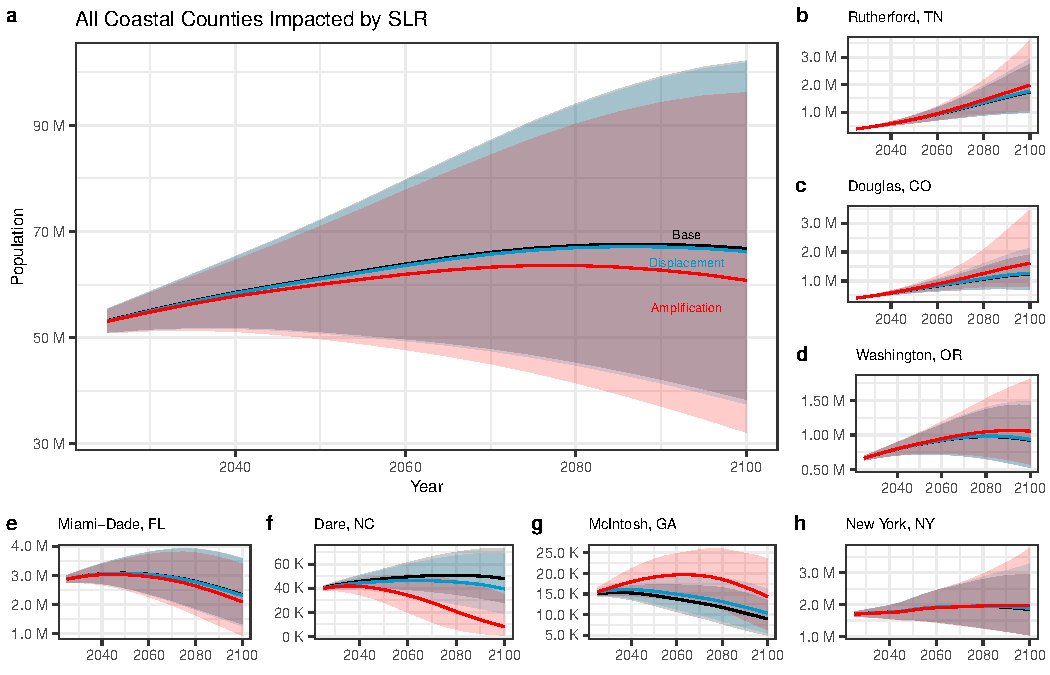
\includegraphics[width=1\linewidth]{FigProjLines2_uncertainty} \caption{\textbf{A comparison of base, inundation, and migration projections for all US coastal counties impacted by sea-level rise and other example counties over the next century.} These projections use RCP4.5. Uncertainty reflects the 95th percentile prediction interval and the minimum/maximum SSP. We adopt the general climate migration typology as proposed by \citep{marandi2021vulnerable} for the seven example counties. (a) compares the population trajectories for all US coastal counties impacted by SLR. Here we can see the amplification effect of population processes and migration, driving population much lower than a simple displacement model suggests. (b-d) are example `Destination' counties using \citep{marandi2021vulnerable}'s framework. (e-f) are example `Vulnerable' counties, showing significant declines earlier in the century. (g-h) are example `Recipient' counties. The integrated demographic model (Amplification) exhibits significant amplification of the demographic trajectories, depending on the timing and extent of inundation. \label{fig:Lines}}\label{fig:mainfig}
\end{figure}

We find that RCP4.5 compromises the land area home to 8.6M - 28M {[}5.7M
- 53M{]}
\footnote{Unless otherwise stated, uncertainty intervals in parentheses relate to SSP3-RCP4.5 5th percentile and SSP5-RCP4.5 95th percentile.}
people between 2020 and 2100 (\textbf{\autoref{fig:Lines}a} and
\textbf{\autoref{fig:Map}}). In this simple model, the demographic
impact of SLR manifests as 0.4M - 10M people migrating to other places
for a net demographic change of 0.4M - 10M people (`Displacement'
model). However, when one accounts for population dynamics
(`Amplification' model), the actual \textit{demographic} impact of 0.4M
- 10M migrants is 8.6M - 28M. This is due to two interacting effects: a
compounding or `domino effect' where destination counties attract more
people over time and origin counties attract less and the interaction of
migrants with the other demographic component processes of fertility and
mortality. This total demographic effect is considerably more pronounced
than the simple displacement effect -- 5.3 to 18 times larger. Under all
plausible RCP-SSP scenarios except RCP4.5-SSP3, SLR leads to a
demographic amplification of at least 10 million persons
(\textbf{\autoref{table1}}.

\begin{figure}
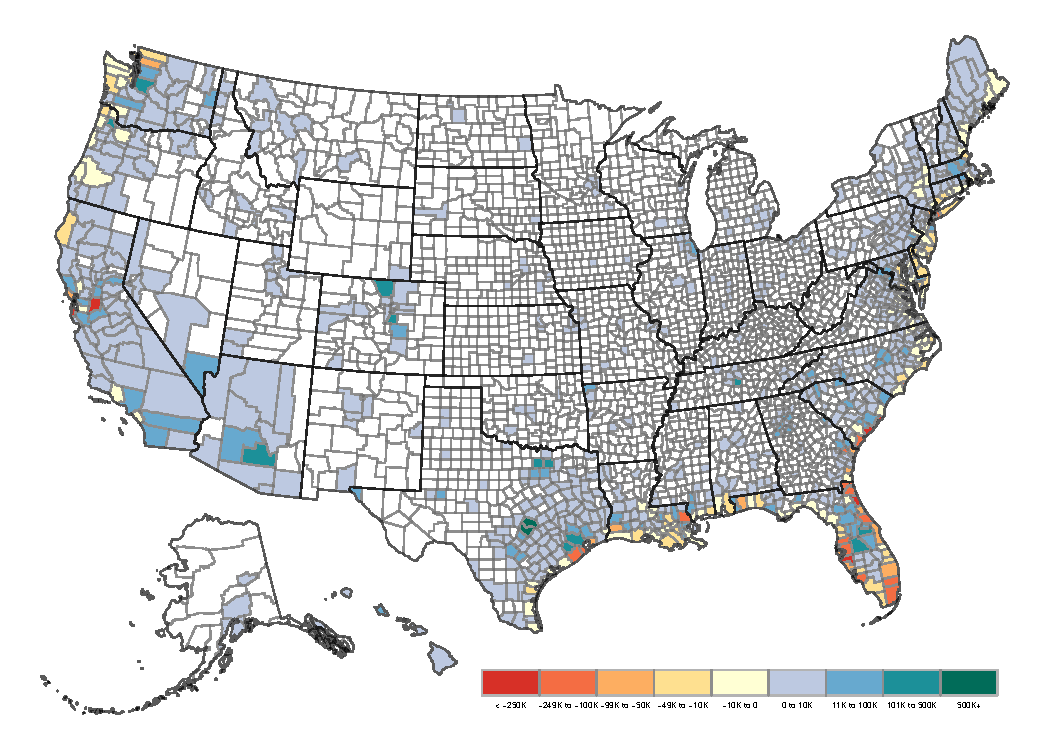
\includegraphics[width=1\linewidth]{FigMedAgeMap3} \caption{\textbf{Projected numeric change in population due to amplified population processes under SSP2-RCP4.5 50th percentile in 2100.} This map highlights the `domino effect' where climate migration further enhances migration to destinations and suppressing migration to origins. \label{fig:Map}}\label{fig:figmap}
\end{figure}

\begin{table}

\centering 
\caption{\textbf{RCP-SSP matrix for 2100 showing all feasible RCP-SSP combinations} \citep{o2016scenario}. Here we compare the expected number of migrants with the demographic amplification for all reasonable RCP-SSP combinations. All numbers in parentheses are the 90th percentile prediction interval. Regardless of the RCP-SSP combination, matrix population models suggest millions of people will shift in the United States due to sea-level rise.}
\resizebox{\linewidth}{!}{ 
\begin{tabular}{cllllll}\label{table1}
 \textbf{RCP} & \textbf{}           & \textbf{SSP1}        & \textbf{SSP2}        & \textbf{SSP3}         & \textbf{SSP4}         & \textbf{SSP5}        \\
\hline
\multirow{3}{*}{8.5}             & SLR Amount (meters) & \multicolumn{5}{c}{0.79 {[}0.52 - 1.2{]}}   \\
                                 & Migrants (millions)           &                      &                      &                       &                       & 3.4 {[}1.3 - 10{]}   \\
                                 & Demographic Amplification (millions)           &                      &                      &                       &                       & 28 {[}17 - 53{]}     \\
                                 \midrule
\multirow{3}{*}{4.5}             & SLR Amount (meters) & \multicolumn{5}{c}{0.59 {[}0.36 - 0.93{]}}                         \\
                                 & Migrants (millions)          & 1.5 {[}0.65 - 4.2{]} & 1.5 {[}0.63 - 4.1{]} & 0.84 {[}0.36 - 2.3{]} & 1.2 {[}0.51 - 3.3{]}  & 2.2 {[}0.96 - 6.2{]} \\
                                 & Demographic Amplification (millions)            & 15 {[}10 - 27{]}     & 15 {[}10 - 26{]}     & 8.6 {[}5.7 - 15{]}    & 12 {[}8 - 21{]}       & 23 {[}15 - 41{]}     \\ \midrule
\multirow{3}{*}{2.6}             & SLR Amount (meters) & \multicolumn{5}{c}{0.5 {[}0.29 - 0.82{]}}             \\
                                 & Migrants (millions)         & 1.2 {[}0.55 - 3.5{]} & 1.2 {[}0.54 - 3.4{]} &                       & 0.96 {[}0.44 - 2.8{]} & 1.8 {[}0.82 - 5.1{]} \\
                                 & Demographic Amplification (millions)            & 14 {[}9.7 - 24{]}    & 14 {[}9.5 - 24{]}    &                       & 11 {[}7.6 - 19{]}     & 21 {[}15 - 37{]}\\                                    
\hline

\end{tabular}
}
\end{table}

Furthermore, \textbf{\autoref{fig:Lines}} shows this population
compounding effect for seven example counties following the general
typology of climate migration put forth by
\citep{marandi2021vulnerable}. Here, \textbf{\autoref{fig:Lines}e-f} are
counties experiencing significant population declines over the entire
time horizon. Our results for Miami-Dade FL under RCP4.5 suggests
28.3K [4.4K - 204.2K]{} migrants by 2100 but a total demographic impact
of 243.9K [72.9K - 1.1M]{} fewer people. We see similar results for Dare
NC as well (8.5K [1.5K - 22.9K]{} migrants and a 39.8K [14.6K - 70.0K]{}
total demographic impact).

\textbf{\autoref{fig:Lines}g-h} are counties close to heavily threatened
areas. We see two separate population trajectories and demonstrate the
amplification of population change. McIntosh GA is initially a `climate
destination', as people from nearby heavily effected areas migrate into
nearby counties. But as the century wears on, this `climate destination'
turn into a vulnerable county and migration begins to turn into negative
population growth. The difference between the simple, `Displacement'
model and the demographically integrated `Amplification' model suggests
population growth trajectories in opposing directions, where the
`Displacement' model has McIntosh growing into the end of the century
whereas the `Amplification' model has it declining. These results
suggest that many people and their descendants could find themselves
exposed and displaced by SLR as presently safe areas become increasingly
vulnerable over time. In the case of New York NY, SLR initially takes
people away from the county before population growth turns positive in
the tail end of the century, transitioning from a `Vulnerable County' to
a potential `Climate Destination'.

Finally, \textbf{\autoref{fig:Lines}b-d} are examples of `Climate
Destinations' (counties considered `climate havens'). We see a similar,
though reversed, pattern of population trajectories to `Vulnerable
Counties.' Here, Rutherford TN (245.1K [78.5K - 852.3K]{} amplified
demographic change versus 34.9K [8.2K - 197.5K]{} displaced migrants),
Douglas CO (377.7K [117.8K - 1.6M]{} vs.~32.3K [5.2K - 230.3K]), and
Washington OR (131.9K [50.9K - 377.8K]{} vs.~12.9K [3.8K - 55.1K])
exhibit considerably larger demographic impacts when accounting for
population dynamics compared to just the displacement model. These
results echo suggestions of emerging climate havens in `safer' areas
\citep{marandi2021vulnerable}.

\begin{figure}
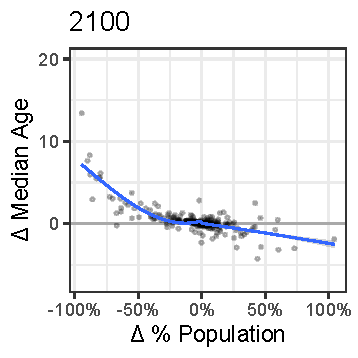
\includegraphics[width=0.7\linewidth]{FigAging3} \caption{\textbf{Population Aging and climate migration}. Here we show he relationship between population decline due to SLR and aging by 2100. The more an area experiences climate out-migration, the greater the population aging. Conversely, the more an area experiences climate in-migration, the younger the area becomes. Results shown are under SSP2-RCP4.5 50th percentile. \label{fig:aging}}\label{fig:figaging}
\end{figure}

\textbf{\autoref{fig:aging}} shows the impact of population processes on
aging related to climate migration. We find that as the percentage of
the population lost due to climate migration-related population
processes increases, the median age in the population also increases
(\textbf{\autoref{fig:aging}}). Conversely, counties receiving the
greatest increase actually exhibit more \emph{youthful} populations.
This effect is particularly pronounced in some counties where the
increase in median age can approach 10+ years in some highly impacted
coastal counties due to climate migration.

\hypertarget{discussion}{%
\section{Discussion}\label{discussion}}

Climate migration continues to receive both policy and scientific focus.
But projections of climate migration that do not account for other
population processes fail to describe compounding population effects or
accelerated population aging in origins. When population processes are
fully integrated within a climate migration model, we see dramatic
impacts on both origin and destination communities, particularly in
their changing age structures.

Given our results, vulnerable areas experiencing climate out-migration
could face a future where more youthful age groups exercise `migration
as adaptation' but the oldest populations remain in vulnerable areas.
Climate migration could place an enormous burden on those communities'
that might face the triple challenges of climate change, dwindling
populations, and rapid population aging. Adaptation costs continue to
rise \citep{buchner2014global} but communities could struggle to afford
the necessary adaptation strategies to protect their remaining residents
as prime-age income earners migrate away, potentially eroding local tax
bases.

Furthermore, given the accelerated population aging in origin
communities, maladaptation could easily result if adaptation strategies
are aimed at more youthful populations who are less likely to remain in
these areas. Some adaptation strategies to build resiliency to SLR call
for raising first floor elevations \citep{dedekorkut2020tide} yet
elevating homes and adding steps might result in maladaptation in
communities facing accelerated aging due to climate migration.

Destination communities also face challenges due to climate migration.
Destination communities that only consider climate migrants
underestimate the population change likely to occur due to demographic
compounding effects. Climate destinations are likely to become even more
attractive as additional gravity driven migration effects play a crucial
factor for additional migration streams, beyond just climate migrants.
For some climate destinations already struggling with growth management
and sustainability goals, climate migration poses significant
challenges. The total demographic impact of climate migration could
further burden these communities if growth is managed haphazardly.
Destination communities for climate migrants should consider these other
demographic forces in their sustainability plans and address challenges
sooner rather than later.

Climate migration has been broadly conceptualized as simply a
rearrangement of people across space. Our results show that this
conceptualization underestimates the total demographic impact in two
main ways: climate migration is likely to accelerate population aging in
origins and accelerate population growth in destinations. We also
demonstrate that climate migration in isolation is unlikely to
significantly alter population distributions but climate migration in
combination with other population processes \emph{will} produce
significant demographic shifts in the future. This work offers the first
glimpse of these demographic shifts.

We model RCPs 2.6, 4.5, and 8.5 which imply a maximum 2100 SLR amount at
1.2m under RCP8.5 \citep{koppProbabilistic21st22nd}. While these SLR
amounts are in line with recent IPCC projections, other SLR projections
suggest 2100 SLR could greatly exceed 1.2m
\citep[\citet{bamber2019ice},\citet{sweetGlobalRegionalSea2017}]{rahmstorfSemiEmpiricalApproachProjecting2007}.
It is possible that the demographic amplification we find is likely
conservative. We also choose to model migration resulting from complete
inundation yet it is possible migration begins sooner than complete
inundation \citep{hauer2020sea}. Thus, the direct migration we model
could also be considered conservative. If people migrate sooner, in a
more anticipatory manner, the demographic amplification we find would be
understated. --\textgreater{}

Additionally, the approach for modeling the demographic implications of
climate migration shown here allows for modelling demographic change in
concert with other climate stressors -- not just SLR. Our parsimonious,
one-dimensional displacement model requires minimal translation of
climate hazards into age-specific displacement. Future scientists could
implement extreme heat/humidity combinations, tropical cyclones, or
water availability as either singular climate hazards or in a
multi-hazard model. To our knowledge, few, if any, demographic
projection models account for climate change impacts. This type of
modelling approach has great potential to better understand the
integration of population processes and climate change.

\hypertarget{acknowledgements}{%
\section{Acknowledgements}\label{acknowledgements}}

This work was supported by the State of Louisiana, the American Society
of Adaptation Professionals, the New York State Energy Research \&
Development Authority, and the Great Lakes Integrated Sciences \&
Assessment. We would like to thank T. Gill, N. Nagle, A. Moulton, S.
Bohon, C. Schmertmann, and E. Fenimore, for their early feedback and
assistance. Thank you!

\hypertarget{methods-and-materials}{%
\section{Methods and Materials}\label{methods-and-materials}}

We employ the use of multiregional Leslie matrices
\citep{rogers1966multiregional} to project climate migration in the
United States. \textbf{Equation 1} is the general form for our
projections.

To answer our research questions, we employ three main modules. The
first is the development of a parsimonious, one-dimensional,
age-specific displacement model. The second is a sea-level rise exposure
model. The third is a multiregional Leslie matrix specification.

\hypertarget{parimonious-one-dimensional-age-specific-displacement-model}{%
\subsection{Parimonious, one-dimensional, age-specific displacement
model}\label{parimonious-one-dimensional-age-specific-displacement-model}}

Our displacement model makes use of a statistical time series outlier
detection technique to first identify anomalous demographic behavior in
a time series and then verify that this anomalous behavior is associated
with an environmental event.

We use a statistical time series outlier detection algorithm
\citep{chen1993joint}, implemented in the R programming language
\citep{rcore} via the tsoutliers package \citep{tsoutliers2019}.

This algorithm iteratively uses ARIMA models to 1) identify potential
outliers and 2) refit the ARIMA with the outliers removed to produce a
counter-factual time series. First, an ARIMA model is fit to the time
series using the \texttt{forecast} package in R
\citep[\citet{hymdman2008}]{Rforecast} where the best performing ARIMA
model is selected based on the Bayesian information criterion (BIC).
Finally, the residuals from the forecast are checked for their
significance where only outliers above a critical \(t\)-static are
considered ``true'\,' outliers (\(|\tau| \geq 4\); p-value \textless{}
0.000063). We chose this threshold to minimize the probability of
committing a Type I error (or claiming an outlier is true when it is, in
fact, not).

We use this outlier detection algorithm to search over county population
totals for the time period 1980-2019. We use the National Vital
Statistics System (NVSS) U.S. Census Populations with Bridged Race
Categories data set. The NVSS Bridged Race Categories data set
harmonizes racial classifications across disparate time periods to allow
population estimates to be sufficiently comparable across space and
time. Importantly, all county boundaries are rectified to be
geographically consistent across all time periods. We use the the
1969-2019 data set, but the historical population estimates prior to
1980 display unusual volatility, so we consider only the time periods
1980-2019. We also only consider counties created prior to year 2000 and
contained in the NVSS data.

We search all US counties for negative statistical outliers (indicating
population losses) between 1980 and 2019. We detect 52 county-years with
population losses of magnitude 4\(\sigma\) or greater. We then use the
Spatial Hazard Events and Losses Database for the United States
(SHELDUS) \citep{SHELDUS}, a county-level hazard data set for the US
which contains information about the direct losses (property and crop
losses, injuries, and fatalities) caused by a hazard event
(thunderstorms, hurricanes, floods, wildfires, tornadoes, flash floods,
earthquakes, etc.) for the period 1960 to the present. We use SHELDUS to
ensure the county time periods we identify as statistical outliers with
population losses experienced an environmental hazard in that
county-year with per capita hazardous losses in excess of the 50th
percentile. This is to ensure the outlier population losses that we
detect are associated with a hazard rather than other forces, such as
economic forces.

Four county-periods either were not in the SHELDUS database or
experienced per capita hazard losses below the 50th percentile.
Additionally, one county-period contained age-sex groups with 0 people,
necessitating exclusion. The remaining 48 environmental events include
tornadoes, wind damage, winter weather, earthquakes, flooding, tropical
cyclones, hail, and other environmental hazards. Using this universe of
48 county-periods exhibiting large population declines after verified
hazard losses, across over 40 years and across a wide variety of
environmental hazards, we then build a flexible, one-dimensional,
age-specific displacement model.

To link population displacement with age-specific population changes, we
calculate cohort-change ratios (CCRs) in each county using the NVSS
population data for the period 1969-2019. Cohort-change ratios take the
following general form (see
\citep[\citet{swanson2010forecasting}]{hauer2019population} for a more
detailed description):

\[CCR_{x,t}  =  \frac{_nP_{x,t}} {_nP_{x-k,t-k}} \tag{2}\]

Where \(_nP_{x,t}\) is the population aged \(x\) to \(x+n\) in time
\(t\) and \(_nP_{x-k,t}\) is the population aged \(x-k\) to \(x+n-k\) in
time \(t\) where \(k\) refers to the time difference between time
periods. Since mortality must decrement a population, any CCR above 1.0
implies a net-migration rate in excess of the mortality rate, and a
growing population. There is special consideration for both the initial
age group without a preceding age group and the final, open-ended age
interval without a proceeding age group (see \citep{hauer2019population}
for additional details).

We build the following model based on the relationship between the
change in CCRs at age \(x\), \(\Delta CCR_x = CCR_{x,t} / CCR_{x,t-1}\),
and the percentage decline in the total population compared to the
counter-factual in the outlier detection method,
\(\Delta P_t = \hat{P_t} / P_t\):

\[log(\Delta CCR_x) = a_x + b_xh + c_xh^2 \tag{3}\]

Here, \(h\) is the log(\(\Delta P_t\)) and shows a quadratic
relationship with the logarithm of the change in CCRs by age. \(x\)
refers to five-year age groups: 0-4, 5-9,\ldots, 85+. This is a similar
model and approach to Wilmoth et al.'s \citep{wilmoth2012flexible}
flexible, one-dimensional mortality model based on the similarity
between age-specific mortality rates and infant mortality.
\textbf{Table S1} depicts the correlation coefficients between
log(\(\Delta CCR_x\)) and log(\(\Delta P_t\)). The age groups with the
lowest correlation coefficients are young adult males aged 20-39 and
those in the open-ended age interval (80+), suggesting these age/sex
groups react to environmental signals the least predictably.

Using \(h_{ty}=log(\Delta P_{ty})\), we can estimate age-specific
changes in CCRs after an environmental event by simply applying the
following formula:

\begin{equation}
    \hat{CCR_{xy,t}} = CCR_{x,t-1} \cdot e^{\hat\beta_xh_{ty}+\hat c_xh^2_{ty}} \label{eq:migmodel}
\end{equation}

Where \(e^{\hat\beta_xh_{ty}+\hat c_xh^2_{ty}}\) provides the percentage
change in \(CCR_{xt}\) based on the log(\(\Delta{P_{ty}}\)) under SLR
amount \(y\). In this case, we drop the intercept (\(a_x\)) from the
estimation procedure to ensure a 0\% decline in population yields a
corresponding 0\% change in the CCR. Multiplying the result from the
model with the CCR in the year prior yields the anticipated change in
the CCR. These changes in CCRs can then be applied to any time series of
population values to generate an anticipated population.

We estimate the predicted population using the equation outlined above
and then compare it against the observed population.
\textbf{Figures S1, S2}, and \textbf{Table S1} show the accuracy of our
fitted, one-dimensional model. Regarding the total population in our 48
counties, our model performs well with an \(r^2\) value of 0.996 and
performs well regardless of population size. Regarding each individual
\(P_x\) group, our model still performs quite well with an \(r^2\) of
0.995. Just like with the total population, the accuracy of our model
does not depend on population size.

\hypertarget{sea-level-rise-exposure}{%
\subsection{Sea-level Rise Exposure}\label{sea-level-rise-exposure}}

To estimate the populations at-risk to SLR and thus the value \(h\) in
\autoref{eq:migmodel}, we employ inundation modeling
\citep{hauer2020sea} which assumes that people who are underwater 100\%
of the time must migrate. We estimate these populations using airborne
lidar-derived digital elevation models (DEMs) produced by NOAA and
supplemented with both the USGS Northern Gulf of Mexico Topobathymetric
DEM in Louisiana and the USGS National Elevation Dataset in the fraction
of land not covered by other sources (see \citep{kulp2019new} for
details on the construction of the DEMs).

Using a bathtub model of inundation, we calculate the land area under a
given water height to generate binary inundation surfaces. SLR exposure
is hyperlocalized and we generate this inundation area in the Census
Block Groups (CBG; n=81,815) located in coastal counties (n=406)
expected to experience any probability of flooding. We use probabilistic
SLR projections
\citep{sweetGlobalRegionalSea2017, koppProbabilistic21st22nd2014} that
are closely aligned with the IPCC for our water heights. To calculate
the land area under a given water height, we simply threshold the DEM to
find pixels below \(SLR_{yt}\) where \(y\) is the projected height of
SLR in a given year \(t\). For each CBG, we simply calculate the
percentage of its pixels on dry land (defined in the National Wetland
Inventory \citep{WetlandInventory}) covered by the inundation surface
and multiply this percentage by the total population in the CBG in year
\(t\) to produce the total number of people at-risk to a given amount of
SLR in a given year. We then aggregate these CBGs to the county-level to
calculate the percentage of people in a given county at-risk of
inundation.

To account for potential sub-county shifts in population, we use the
specification of sub-county demographic projections
\citep{hauerMillionsProjectedBe2016}. Specifically, we use a sub-county
demographic projection to produce spatiotemporally consistent CBG
boundaries for the period 1940-2010 and project these populations
forward using a mixed, linear/exponential projection for the period
2010-2100. CBGs expected to increase use a linear projection and CBGs
expected to decrease use an exponential projection. This creates a
time-varying, population-weighted estimate of exposure to SLR.

The percentage of the population at-risk to SLR in each county, in
essence, represents the \(\Delta P_t\) from our \autoref{eq:migmodel}
above where \(\Delta P_t = P_{t,y}/P_t\). In this case, \(P_{t,y}/P_t\)
is the percentage of the population in any county at-risk of inundation
under a given water height \(y\). Such a calculation allows us to
seamlessly combine our parsimonious displacement model with our matrix
population model.

\hypertarget{matrix-population-models}{%
\subsection{matrix Population Models}\label{matrix-population-models}}

We employ the use of multiregional Leslie matrices in our population
projections \citep{rogers1966multiregional}.

Where \(\mathbf{P}_t\) refers to the population matrix containing \(x\)
age groups and \(\mathbf{S}_t\) contains the age-specific fertility
(\(F\)) and mortality rates (\(S\)), where \(S_x\) refers to the
survival probabilities for age group \(x\) and \(F_x\) refers to the
fertility rates.

We populate our Leslie matrices with the 3,143 US counties, 18 five-year
age groups, and two sex groups, thus, \(\mathbf{P}_t\) is a vector of
length 113,148, and \(\mathbf{S}_t\) and \(\mathbf{M}_{ty}\) are 113,148
x 113,148 matrices. We use CCRs to populate our \(S_x\) values in each
matrix and child-woman ratios to populate our \(F_x\) values. The values
come from the NVSS Bridged Race Categories dataset. To project the CCRs,
We employ an autoregressive integrated moving average (ARIMA) model for
forecasting equally spaced univariate time series data. We use an
\texttt{ARIMA(0,1,1)} model, which produces forecasts equivalent to
simple exponential smoothing. All projections were undertaken in
\textit{R} \citep{rcore} using the \texttt{forecast} package
\citep{Rforecast}.

We use the NVSS data for the period 1969-2019 for county \(c\), age
group \(x\), sex \(s\) in an \texttt{ARIMA(0,1,1)} to create
\(CCR_{cxst}\) for time periods \(t+1\). The initial \(\mathbf{P}_1\)
and \(\mathbf{S}_t\) matrices use the 2019 NVSS data.

We also calculate the probability of migrating from each county to each
county and use this to populate the \(\mathbf{M}_{ty}\) matrix. These
data come from the IRS county-to-county migration files for 1990-2018
(see \citep{hauer2019irs, dewaard2021user} for descriptions of this
data). We populate \(\mathbf{M}_{ty}\) as
\(M_t\cdot(1-e^{\hat\beta_xh_{ty}+\hat c_xh^2_{ty}})\) and where \(i=j\)
as \(e^{\hat\beta_xh_{ty}+\hat c_xh^2_{ty}}\). \(M_t\) is a vector
containing the proportion migrating from county \(i\) to county \(j\) in
the IRS migration data, thus ensuring the columns of \(\mathbf{M}_{ty}\)
sum to 1.0.

To capture changes in the migration system, we employ an ETS model
(Error, Trend, Seasonal), a univariate time series forecasting model
\citep{hyndman2008forecasting}. We use an ETS model for migration
instead of an ARIMA(0,1,1) as we do for the CCRs because the CCRs are
subject to multiplication during a drift, whereas the migration system
is not. A CCR that drifts from 1.1 \(\rightarrow\) 1.3 represents more
than a 10-fold increase in a projected population over our time horizons
(\(1.1^{17}\) = 5x, \(1.3^{17}\) = 86x). Projecting the migration system
itself is not subject to such exponential drift.

We fit individual ETS models for each county's numeric migrants between
each origin-destination dyadic pair using the \texttt{forecast} package
in R \citep{Rforecast}. This approach allows the underlying migration
system to evolve and change over the projection horizon, allowing dyadic
pairs to wax or wane. We convert the numeric projections to fractions of
the total projected migrants to populate the diagonal in the
\(\mathbf{M}\) matrix above where non-migrants (i.e.~those migrating
from \(i\rightarrow i\)) are included. The result is the fraction of
individuals surviving from age group \(x\) who migrate from
\(i\rightarrow j\).

We control all population projections to the Shared Socioeconomic
Pathways \citep{samir2017human} and we use RCPs 2.6, 2.5, and 8.5 for
our inundation scenarios \citep{koppProbabilistic21st22nd2014}.

\clearpage

\hypertarget{supplementary-information}{%
\section{Supplementary Information}\label{supplementary-information}}

\begin{table}

\caption{\textbf{Correlation coefficients of changes in Cohort Change Ratios vs. Total Population Change (n=48).}}
\centering
\begin{tabular}[t]{lrr}
\toprule
Age Group & Male & Female\\
\midrule
0-4 & 0.932 & 0.944\\
5-9 & 0.959 & 0.934\\
10-14 & 0.963 & 0.962\\
15-19 & 0.805 & 0.925\\
20-24 & 0.656 & 0.919\\
\addlinespace
25-29 & 0.710 & 0.932\\
30-34 & 0.754 & 0.957\\
35-39 & 0.870 & 0.974\\
40-44 & 0.927 & 0.960\\
45-49 & 0.966 & 0.958\\
\addlinespace
50-54 & 0.963 & 0.972\\
55-59 & 0.962 & 0.956\\
60-64 & 0.894 & 0.890\\
65-69 & 0.813 & 0.916\\
70-74 & 0.934 & 0.824\\
\addlinespace
75-79 & 0.840 & 0.802\\
80+ & 0.466 & 0.646\\
\bottomrule
\end{tabular}\label{CorTable}
\end{table}

\begin{figure}
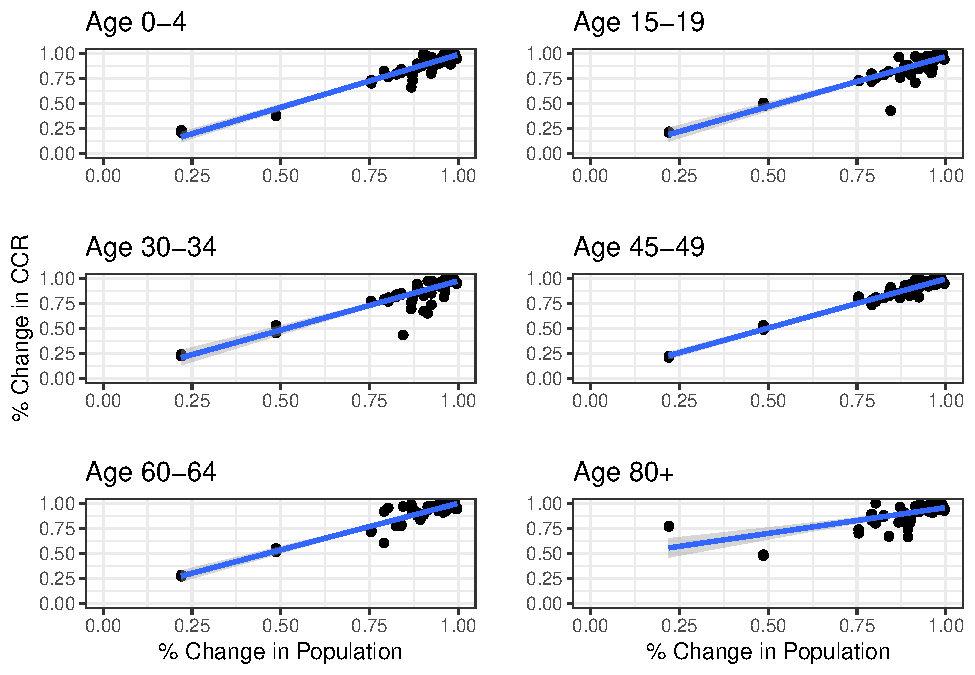
\includegraphics[width=1\linewidth]{CCRfig-1} \caption{\textbf{Age-specific changes in cohort-change ratios vs. change in total population for selected age groups.} \label{fig:Ageresults}}\label{fig:figagemodel}
\end{figure}

\begin{figure}
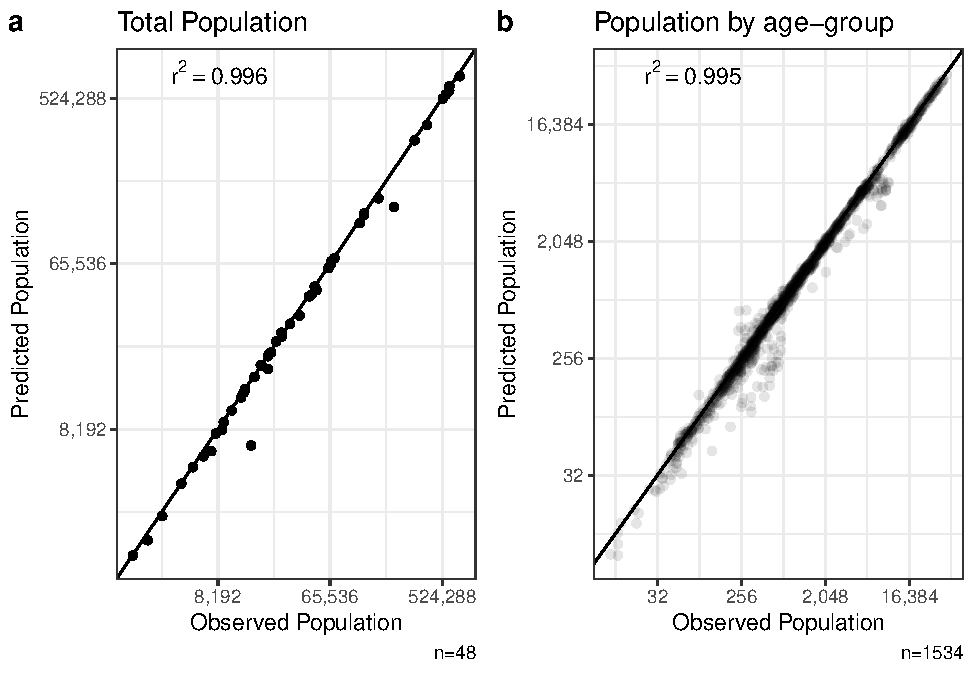
\includegraphics[width=1\linewidth]{evalfig-1} \caption{\textbf{Relationship between predicted populations using our model and observed populations in the 48 counties in our selection.} (a) shows the total population and (b) shows the populations for each age/sex group. The diagonal solid line is y=x. The model produces good fits for both the total population and by age/sex group. \label{EvalFig}}\label{fig:figeval}
\end{figure}

\hypertarget{matrix-population-projections}{%
\subsection{Matrix Population
Projections}\label{matrix-population-projections}}

To investigate SLR migration, we produce three separate population
projections using a multi-regional Leslie matrix that takes the
following general form

\begin{equation}
 \begin{array}{lll}
\text{Base}          &: \mathbf{P}_{t+1}^{Base} & =\mathbf{S}_t\mathbf{P}_t^{Base}\\
\text{Displacement}  &: \mathbf{P}_{t+1}^{Disp} &= \mathbf{M}_{ty}\mathbf{S}_{t}\mathbf{P}_t^{Base} \\
\text{Amplification} &: \mathbf{P}_{t+1}^{Amp}  &=\mathbf{M}_{ty}\mathbf{S}_{t}\mathbf{P}_t^{Amp}
\end{array}
\end{equation}

In this section, we provide examples for all three projections. We will
use a simplified example for a two-region population containing three
age groups where each age group in region 1 contains 100 individuals and
each age group in region 2 contains 200 individuals.

\hypertarget{base-projection}{%
\subsubsection{Base Projection}\label{base-projection}}

We employ the use of multiregional leslie matrices in our population
projections.

In a typical Leslie matrix, \begin{equation}
    \mathbf{P}_{t+1} = \mathbf{S}_t \cdot \mathbf{P}_t \label{eq:lesliematrix_base} \tag{5} \nonumber
\end{equation}

Where \(\mathbf{P}_t\) refers to the population vector containing \(x\)
age groups and \(\mathbf{S}_t\) contains the age-specific fertility and
mortality rates.

In a population with three age groups, production of a population
projection looks akin to

\begin{equation}
\mathbf{P}_{t+1} =
\begin{bmatrix}
    0 & F_2 & F_3 \\
    S_1 & 0 & 0 \\
    0 & S_2 & S_3
\end{bmatrix}
\cdot
\begin{bmatrix}
    P_1 \\
    P_2 \\
    P_3
\end{bmatrix}\nonumber
\end{equation}

where \(S_x\) refers to the survival probabilities for age group \(x\)
and \(F_x\) refers to the fertility rates. In practice, we populate
\(S_x\) using cohort-change ratios described in the Main Text.

These two matrices (\(\mathbf{S}_t\) and \(\mathbf{P}_t\)) for our
example populations take the following forms.

\begin{equation}
\mathbf{P}_t = 
\begin{bmatrix}
\begin{array}{c}
100 \\
100 \\
100 \\
\hline
200\\
200\\
200\\
\end{array}
\end{bmatrix} 
\end{equation}

\begin{equation}
\mathbf{S}_t =
\begin{bmatrix}
\begin{array}{c|c}
\begin{matrix} 0 & 0.2 & 0.2 \\ 1.05 & 0 & 0 \\ 0 & 0.35 & 0.35 \end{matrix} &
\begin{matrix} 0 & 0 & 0 \\ 0 & 0 & 0 \\ 0 & 0 & 0 \end{matrix} \\
\hline
\begin{matrix} 0 & 0 & 0 \\ 0 & 0 & 0 \\ 0 & 0 & 0 \end{matrix} &
\begin{matrix} 0 & 0.2 & 0.2 \\ 0.98 & 0 & 0 \\ 0 & 0.33 & 0.33 \end{matrix} \\
\end{array}
\end{bmatrix}
\end{equation}

Thus, the `Base' population projection produces

\begin{equation} 
\mathbf{P}_{t+1} =  
\begin{bmatrix}
\begin{array}{c|c}
\begin{matrix} 0 & 0.2 & 0.2 \\ 1.05 & 0 & 0 \\ 0 & 0.35 & 0.35 \end{matrix} &
\begin{matrix} 0 & 0 & 0 \\ 0 & 0 & 0 \\ 0 & 0 & 0 \end{matrix} \\
\hline
\begin{matrix} 0 & 0 & 0 \\ 0 & 0 & 0 \\ 0 & 0 & 0 \end{matrix} &
\begin{matrix} 0 & 0.2 & 0.2 \\ 0.67 & 0 & 0 \\ 0 & 0.33 & 0.33 \end{matrix} \\
\end{array}
\end{bmatrix}
\cdot
\begin{bmatrix}
\begin{array}{c}
100 \\
100 \\
100 \\
\hline
200\\
200\\
200\\
\end{array}
\end{bmatrix} \nonumber
\end{equation}

\begin{equation} 
\mathbf{P}_{t+1} =  \begin{bmatrix}
\begin{array}{c}
40 \\
105 \\
70 \\
\hline
80\\
196\\
132\\
\end{array}
\end{bmatrix} 
\end{equation}

Here we would project region 1's population to go from 300 individuals
in period 1 to 215 individuals in period 2 and region 2's population to
go from 600 individuals to 408.

\hypertarget{displacement-and-amplification-models}{%
\subsubsection{Displacement and Amplification
Models}\label{displacement-and-amplification-models}}

Our Displacement and Amplification models are similar but utilize
multiregional Leslie matrices. In a multi-regional projection model, we
can use a ``super-matrix.''

A 2-region model would take the following general form for the
\(\mathbf{S}_t\) matrix, \begin{equation}
 \mathbf{MS}_t =
\begin{bmatrix}
\begin{array}{c|c}

\mathbf{S}_i & \mathbf{M}_{j\rightarrow i} \\
\hline
\mathbf{M}_{i\rightarrow j} & \mathbf{S}_j \\


\end{array}
\end{bmatrix}
\nonumber
\end{equation}

Such that the diagonal \(\mathbf{S}\) matrices contain combined
survival, fertility, and migration probabilities while the off-diagonal
\(\mathbf{M}\) matrices contain the probabilities of each age-group
moving from one region \(i\) to region \(j\).

Here, we use the population vector resulting from the \(Base\)
projection for our Displacement model and a new matrix,
\(\mathbf{M}_{ty}\), which contains the probability of migrating from
one region to another. In a two region projection, 100\% of migrants
move from region 1 to region 2 and vice versa and 0\% of migrants are
non-movers (ie, region \(1\rightarrow\) region \(1\)). For this example,
Region 1 experiences 10\% of its land area inundated by SLR (\(h\) =
0.10) and Region 2 experiences 0\% of its land inundated by SLR. We
populate the diagonal with the result of the parsimonious displacement
model but for illustrative purposes, we assume that the result is equal
to \(h\). In practice, the value depends on both \(h\) and the specific
age group \(x\), ultimately resulting from
\(e^{\hat\beta_xh_{ty}+\hat c_xh^2_{ty}}\).

\begin{equation}
\mathbf{M}_{ty} =
\begin{bmatrix}
\begin{array}{c|c}
\begin{matrix} 0.9 & 0 & 0 \\ 0 & 0.9 & 0 \\ 0 & 0 & 0.9 \end{matrix} &
\begin{matrix} 0 & 0 & 0 \\ 0 & 0 & 0 \\ 0 & 0 & 0 \end{matrix} \\
\hline
\begin{matrix} 0.1 & 0 & 0 \\ 0 & 0.1 & 0 \\ 0 & 0 & 0.1 \end{matrix} &
\begin{matrix} 1 & 0 & 0 \\ 0 & 1 & 0 \\ 0 & 0 & 1 \end{matrix} \\
\end{array}
\end{bmatrix}
\end{equation}

Multiplying \(\mathbf{M}_{ty}\) with \(\mathbf{S}_t\) produces a
combined migration/survival matrix that when multiplied by
\(\mathbf{P}_t\) yields the projected population.

\begin{equation}
\mathbf{M}_{ty}\mathbf{S}_t = 
\begin{bmatrix}
\begin{array}{c|c}

\begin{matrix} 0 & 0.18 & 0.18 \\ 0.945 & 0 & 0 \\ 0 & 0.315 & 0.315 \end{matrix} &
\begin{matrix} 0 & 0 & 0 \\ 0 & 0 & 0 \\ 0 & 0 & 0 \end{matrix} \\
\hline
\begin{matrix} 0 & 0.02 & 0.02 \\ 0.105 & 0 & 0 \\ 0 & 0.035 & 0.035  \end{matrix} &
\begin{matrix} 0 & 0.2 & 0.2 \\ 0.98 & 0 & 0 \\ 0 & 0.33 & 0.33 \end{matrix} \\
\end{array}
\end{bmatrix}
\end{equation}

\begin{equation}
\mathbf{P}_{t+1} = 
\begin{bmatrix}
\begin{array}{c|c}

\begin{matrix} 0 & 0.18 & 0.18 \\ 0.945 & 0 & 0 \\ 0 & 0.315 & 0.315 \end{matrix} &
\begin{matrix} 0 & 0 & 0 \\ 0 & 0 & 0 \\ 0 & 0 & 0 \end{matrix} \\
\hline
\begin{matrix} 0 & 0.02 & 0.02 \\ 0.105 & 0 & 0 \\ 0 & 0.035 & 0.035  \end{matrix} &
\begin{matrix} 0 & 0.2 & 0.2 \\ 0.98 & 0 & 0 \\ 0 & 0.33 & 0.33 \end{matrix} \\
\end{array}
\end{bmatrix}
\cdot
\begin{bmatrix}
\begin{array}{c}
100 \\
100 \\
100 \\
\hline
200\\
200\\
200\\
\end{array}
\end{bmatrix}
=
\begin{bmatrix}
\begin{array}{c}
36 \\
94.5\\
63 \\
\hline
84\\
206.5\\
139\\
\end{array}
\end{bmatrix}
\end{equation}

Note: Our Displacement model uses \(\mathbf{P}_t^{Base}\) rather than
\(\mathbf{P}_t^{Disp}\). This renders our projected climate migrants
demographically inert with no interaction with future component
processes.

Our Amplification model differs in only a single way from our
Displacement model. Rather than using \(\mathbf{P}_t^{Base}\), this
model uses \(\mathbf{P}_t^{Amp}\), allowing all projected climate
migrants to demographically interact with future component processes.

\bibliographystyle{agsm}
\bibliography{bibliography.bib}


\end{document}
